\def\year{2021}\relax
%File: formatting-instructions-latex-2021.tex
%release 2021.1
\documentclass[letterpaper]{article} % DO NOT CHANGE THIS
\usepackage{aaai21}  % DO NOT CHANGE THIS
\usepackage{times}  % DO NOT CHANGE THIS
\usepackage{helvet} % DO NOT CHANGE THIS
\usepackage{courier}  % DO NOT CHANGE THIS
\usepackage[hyphens]{url}  % DO NOT CHANGE THIS
\usepackage{graphicx} % DO NOT CHANGE THIS
\usepackage{subfigure}
\urlstyle{rm} % DO NOT CHANGE THIS
\def\UrlFont{\rm}  % DO NOT CHANGE THIS
\usepackage{natbib}  % DO NOT CHANGE THIS AND DO NOT ADD ANY OPTIONS TO IT
\usepackage{caption} % DO NOT CHANGE THIS AND DO NOT ADD ANY OPTIONS TO IT
\frenchspacing  % DO NOT CHANGE THIS
\setlength{\pdfpagewidth}{8.5in}  % DO NOT CHANGE THIS
\setlength{\pdfpageheight}{11in}  % DO NOT CHANGE THIS
%\nocopyright
%PDF Info Is REQUIRED.
% For /Author, add all authors within the parentheses, separated by commas. No accents or commands.
% For /Title, add Title in Mixed Case. No accents or commands. Retain the parentheses.
\pdfinfo{
/Title (Generalized Out-of-distribution Indicator via Deep Generative Models)
/Author (Wenxiao Chen, Xiaohui Nie, Mingliang Li, Dan Pei)
/TemplateVersion (2021.1)
} %Leave this
% /Title ()
% Put your actual complete title (no codes, scripts, shortcuts, or LaTeX commands) within the parentheses in mixed case
% Leave the space between \Title and the beginning parenthesis alone
% /Author ()
% Put your actual complete list of authors (no codes, scripts, shortcuts, or LaTeX commands) within the parentheses in mixed case.
% Each author should be only by a comma. If the name contains accents, remove them. If there are any LaTeX commands,
% remove them.

% DISALLOWED PACKAGES
% \usepackage{authblk} -- This package is specifically forbidden
% \usepackage{balance} -- This package is specifically forbidden
% \usepackage{color (if used in text)
% \usepackage{CJK} -- This package is specifically forbidden
% \usepackage{float} -- This package is specifically forbidden
% \usepackage{flushend} -- This package is specifically forbidden
% \usepackage{fontenc} -- This package is specifically forbidden
% \usepackage{fullpage} -- This package is specifically forbidden
% \usepackage{geometry} -- This package is specifically forbidden
% \usepackage{grffile} -- This package is specifically forbidden
% \usepackage{hyperref} -- This package is specifically forbidden
% \usepackage{navigator} -- This package is specifically forbidden
% (or any other package that embeds links such as navigator or hyperref)
% \indentfirst} -- This package is specifically forbidden
% \layout} -- This package is specifically forbidden
% \multicol} -- This package is specifically forbidden
% \nameref} -- This package is specifically forbidden
% \usepackage{savetrees} -- This package is specifically forbidden
% \usepackage{setspace} -- This package is specifically forbidden
% \usepackage{stfloats} -- This package is specifically forbidden
% \usepackage{tabu} -- This package is specifically forbidden
% \usepackage{titlesec} -- This package is specifically forbidden
% \usepackage{tocbibind} -- This package is specifically forbidden
% \usepackage{ulem} -- This package is specifically forbidden
% \usepackage{wrapfig} -- This package is specifically forbidden
% DISALLOWED COMMANDS
% \nocopyright -- Your paper will not be published if you use this command
% \addtolength -- This command may not be used
% \balance -- This command may not be used
% \baselinestretch -- Your paper will not be published if you use this command
% \clearpage -- No page breaks of any kind may be used for the final version of your paper
% \columnsep -- This command may not be used
% \newpage -- No page breaks of any kind may be used for the final version of your paper
% \pagebreak -- No page breaks of any kind may be used for the final version of your paperr
% \pagestyle -- This command may not be used
% \tiny -- This is not an acceptable font size.
% \vspace{- -- No negative value may be used in proximity of a caption, figure, table, section, subsection, subsubsection, or reference
% \vskip{- -- No negative value may be used to alter spacing above or below a caption, figure, table, section, subsection, subsubsection, or reference

\usepackage{amsmath}
\usepackage{amssymb}
\usepackage{cleveref}

\newtheorem{theorem}{Theorem}
\newtheorem{lemma}{Lemma}
\newtheorem{proof}{Proof}[section]

\newcommand{\IE}{\textit{i.e.}, }
\newcommand{\EG}{\textit{e.g.}, }
\newcommand{\ET}{\textit{et al.}}
\newcommand{\ST}{\textit{s.t.}}


\newcommand{\dd}{\mathrm{d}}
\newcommand{\vv}[1]{\bm{\mathrm{{#1}}}}
\newcommand{\E}{\operatorname{\mathbb{E}}}
\newcommand{\pin}{p_{in}}
\newcommand{\pout}{p_{out}}
\newcommand{\pmix}{p_{mix}}



\setcounter{secnumdepth}{1} %May be changed to 1 or 2 if section numbers are desired.

% The file aaai21.sty is the style file for AAAI Press
% proceedings, working notes, and technical reports.
%

% Title

% Your title must be in mixed case, not sentence case.
% That means all verbs (including short verbs like be, is, using,and go),
% nouns, adverbs, adjectives should be capitalized, including both words in hyphenated terms, while
% articles, conjunctions, and prepositions are lower case unless they
% directly follow a colon or long dash

\title{Generalized Out-of-distribution Indicator via Deep Generative Models}
\author{
    %Authors
    % All authors must be in the same font size and format.
%    Wenxiao Chen, Xiaohui Nie, Mingliang Li, Dan Pei
}
\affiliations{
    %Afiliations

%    Department of Computer Science and Technology, Tsinghua University
%    China Unicom
	
    %If you have multiple authors and multiple affiliations
    % use superscripts in text and roman font to identify them.
    %For example,

    % Sunil Issar, \textsuperscript{\rm 2}
    % J. Scott Penberthy, \textsuperscript{\rm 3}
    % George Ferguson,\textsuperscript{\rm 4}
    % Hans Guesgen, \textsuperscript{\rm 5}.
    % Note that the comma should be placed BEFORE the superscript for optimum readability

    % email address must be in roman text type, not monospace or sans serif
%    chen-wx17@mails.tsinghua.edu.cn

    % See more examples next
}
\iffalse
%Example, Single Author, ->> remove \iffalse,\fi and place them surrounding AAAI title to use it
\title{My Publication Title --- Single Author}
\author {
    % Author
    Author Name \\
}

\affiliations{
    Affiliation \\
    Affiliation Line 2 \\
    name@example.com
}
\fi

\iffalse
%Example, Multiple Authors, ->> remove \iffalse,\fi and place them surrounding AAAI title to use it
\title{My Publication Title --- Multiple Authors}
\author {
    % Authors

        First Author Name,\textsuperscript{\rm 1}
        Second Author Name, \textsuperscript{\rm 2}
        Third Author Name \textsuperscript{\rm 1} \\
}
\affiliations {
    % Affiliations
    \textsuperscript{\rm 1} Affiliation 1 \\
    \textsuperscript{\rm 2} Affiliation 2 \\
    firstAuthor@affiliation1.com, secondAuthor@affilation2.com, thirdAuthor@affiliation1.com
}
\fi
\begin{document}

\maketitle

\begin{abstract}

We consider the problem of detecting out-of-distribution images by deep generative models. We reviewed the recent researches about out-of-distribution based on deep generative models and found a critical weakness that the number of datasets in these works is not enough to support the generality of their indicators. 
Therefore, we do a large-scale research for these indicators on more datasets and find that the performance of these indicators is as not well as they claim on large-scale datasets. 
We propose the native indicators based on Kullback–Leibler divergence and Wasserstein distance for detecting out-of-distribution. 
Our indicators are general with solid theoretical basis and proven to be better than log-likelihood indictor, which is expected to guide the development of deep generative models in OoD domain. 
Our indicators outperform past works by a large margin. Moreover, we test our indicators under other limitations to show that our indicators are not data-specific and can be deployed on online system. 
 
\end{abstract}

\section{Introduction}
Machine learning has achieved impressive success in classification domain through deep neural network classifiers. However, these classifiers can be easily fooled by the data from other datasets (called out-of-distribution OoD)~\cite{nguyen2015deep}, which might lead to potential risks in practice. It is necessary to detect OoD data to ensure that applications based on classifiers are robust and stable. Ostensibly, it is intuitive to train a density model $p_\theta(x)$ to approximate the empirical distribution of training data, and refuse the sample $x$ when $p_\theta(x)$ is sufficiently low~\cite{bishop1994novelty}. 
Recently, deep generative models are quickly developed and have been able to generate realistic samples, which indicates that deep generative models assign high density to the samples of the training data, and density can be used for detecting out-of-distribution. 

However, contrary to popular belief, recent works~\cite{nalisnick2018deep,choi2018waic,hendrycks2018deep} show that density estimates by deep generative models assign higher density to the most samples from out-of-distribution and fail to detect OoD. This phenomenon occurs in CIFAR (as training dataset) vs SVHN (as out-of-distribution) for different likelihood-based generative models, while the data in CIFAR and SVHN have significant different semantic. 

Alternative indictors based on likelihood estimates have been proposed~\cite{serra2019input,song2017pixeldefend,choi2018waic,ren2019likelihood,song2019unsupervised,che2019deep} to alleviate this issue. However, we found that the datasets considered in these works are quite less, even only CIFAR and SVHN. It is a natural question whether these indictors work well on large-scale datasets, because a robust model should detect samples from any out-of-distribution by the definition of OoD problem. Therefore, we do a large-scale research for these indicators on more datasets and find that the performance of these indicators is as not well as they claim on large-scale datasets. Based on this observation, we argue that the few datasets will cause unreliable evaluation and evaluation on large-scale datasets should be a common sense in OoD domain. 

Based on the observation on large-scale datasets, we found a common phenomenon that $p_\theta$ has a lower density for samples from in-distribution and higher density for samples from out-of-distribution than $p_\omega$, which is trained on the out-of-distribution. 
Based on this phenomenon and theoretical proof, we propose the native KL indictor, $\log p_\theta(x) - \log p_\gamma(x)$ for OoD detection, where $p_\gamma$ is trained on the mixture distribution. Based on the similar theoretical inference, the discriminator in WGAN can also be used for OoD, called native Wasserstein indictor. 

Our indicators outperform past works by a large margin. Moreover, we test our indicators under other limitations to show that our indicators are not data-specific and can be deployed on online system.

The main contributions of this paper are in the following:
\begin{itemize}
	\item We do a large-scale research for these indicators on more datasets and find that the performance of these indicators is as not well as they claim on large-scale datasets. We argue that the few datasets will cause unreliable evaluation and evaluation on large-scale datasets should be a common sense in OoD domain. 
	\item We propose the native indicators based on Kullback–Leibler divergence and Wasserstein distance for detecting out-of-distribution instead traditional likelihood assumption. It is a novel idea for guiding the indictors based on deep generative models. 
	\item Native KL Indictor and Native Wasserstein Indictor outperforms past works by a large margin. They are not data-specific and can be deployed on online system.
\end{itemize}

\section{Background}
Likelihood-based generative models are widely viewed to be robust to detect out-of-distribution samples by the model density intuitively. However, the densities of common likelihood-based models, \EG RealNVP~\cite{dinh2016density}, VAE~\cite{tomczak2018vae,takahashi2019variational} and PixelCNN~\cite{van2016conditional}, have been shown to be problematic for detecting out-of-distributions~\cite{nalisnick2018deep}. 
To solve this problem, some researches proposed some variants of these models for detecting out-of-distribution~\cite{che2019deep} and some researches proposed improved indicator to replace log-likelihood~\cite{serra2019input}. In our paper, we focus on how to improve the indicators based on common models. 

\cite{song2017pixeldefend} considered using permutation tests statistics $T_{perm}(x)$ to determine whether an input $x$ is in out-of-distribution. They use the rank of $p_\theta(x)$ in the training set as out-of-distribution indicators. Both low-likelihood and high-likelihood samples are identified as OoD. It is significantly useful to solve the counterexample of CIFAR-10 vs SVHN in \cite{nalisnick2018deep}. 

\cite{choi2018waic} used Watanabe Akaike Information Criterion (WAIC) based on independently trained model ensembles.
\begin{equation}
	\text{WAIC}(x) = \mathbb{E}_{\theta} [\log p_\theta(x)] - \operatorname{Var}_{\theta} [\log p_\theta(x)]
\end{equation}

\cite{ren2019likelihood} proposed a likelihood ratio indicator for deep generative models. They proposed a background model $p_{\theta_0}(x)$ to capture the general background statistics and a likelihood ratio indicator $LLR(x)$ to captures the significance of the semantics compared to the background model. 
\begin{equation}
LLR(x) = \log p_\theta(x) - \log p_{\theta_0}(x)
\end{equation}

\cite{serra2019input} observed that input complexity excessively affects the generative models' likelihoods. Based on this observation, they proposed an estimation for input complexity $L(x)$, to derive a parameter-free OoD indicator $S(x)$:
\begin{equation}
	S(x) = -\log p_\theta(x) - L(x)
\end{equation}

\cite{song2019unsupervised} observed that on generative models with batch normalization, the estimated likelihood of a batch of OoD samples is much lower than of of in-distribution samples. Meanwhile, the corresponding log-likelihood decreases dramatically for OoD samples, but is relatively stable for in-distribution samples, as the ratio of test samples in a batch increases. Based on the observation, they proposed a permutation test that statics the change of log-likelihood when the ratio of test samples in a batch changes. 

Researches also proposed to use labels (for classification task) to solve OoD. 
\cite{che2019deep} proposed to use conditional deep generative models to verify the predictions of classifier, when the labels of samples are selected by the classifier. \cite{alemi2018uncertainty} models the bottleneck $I(Z;Y)-\beta I(Z;X)$ where $I$ is the mutual information. 
\cite{hendrycks2016baseline,hendrycks2018deep,hsu2020generalized,lee2018simple} proposed to only use classifier for detecting OoD. 

\section{Problem Statement}\label{sec2}

Let $\pin$ and $\pout$ denote two distinct data distribution define on image space $\mathcal{X}$ where $\pin$ is called in-distribution and $\pout$ is called out-of-distribution. 
Let $\pmix$ denote a mixture distribution $\pmix(x) = \alpha \pin(x) + \beta \pout(x)$ where $\alpha + \beta = 1$ and $\alpha, \beta > 0$. 
For samples generated by $\pmix$, they are generated by $\pin$ or $\pout$ and we want to know which of them are generated by $\pin$ while we do not know any information about $\pout$. 

It is important to decide a whether two datasets are distinct when the number of datasets is large. We call two datasets are \textbf{simply-classified} when a common classifier which is trained on the training data of the two datasets for 2-class classification,\IE in-distribution as label 0 and out-of-distribution as label 1, can simply distinguishing the testing data of the two datasets. If two dataset A, B are simply-classified, we will call their distribution is distinct and A vs B (A as in-distribution and B as out-of-distribution) will be an experiment. 

In this paper, we consider the problem of distinguishing the in-distribution and out-of-distribution images on the common deep generative models, \IE VAE, PixelCNN, flow-based models and GANs. To validate the generality of indicators, large-scale common datasets is used in our experiments, including MNIST, FASHION-MNIST, KMNIST, NOT-MNIST, Omniglot, CIFAR-10, CIFAR-100, TinyImagenet, SVHN, iSUN, CelebA, LSUN, Noise and Constant. 

We consider all common metrics, including AUROC, AUPR, AP, FPR@TPR95. AUROC is selected as the major metrics in our paper and other metrics are shown in appendix B. AUROC is a threshold-independent metric~\cite{davis2006relationship} and is widely used in OoD domain. A perfect detector can get AUROC score of 100\%. 

\section{Motivating Observations}\label{sec3}

\begin{figure}[t]
\centering
\subfigure[CIFAR-10 vs SVHN]{
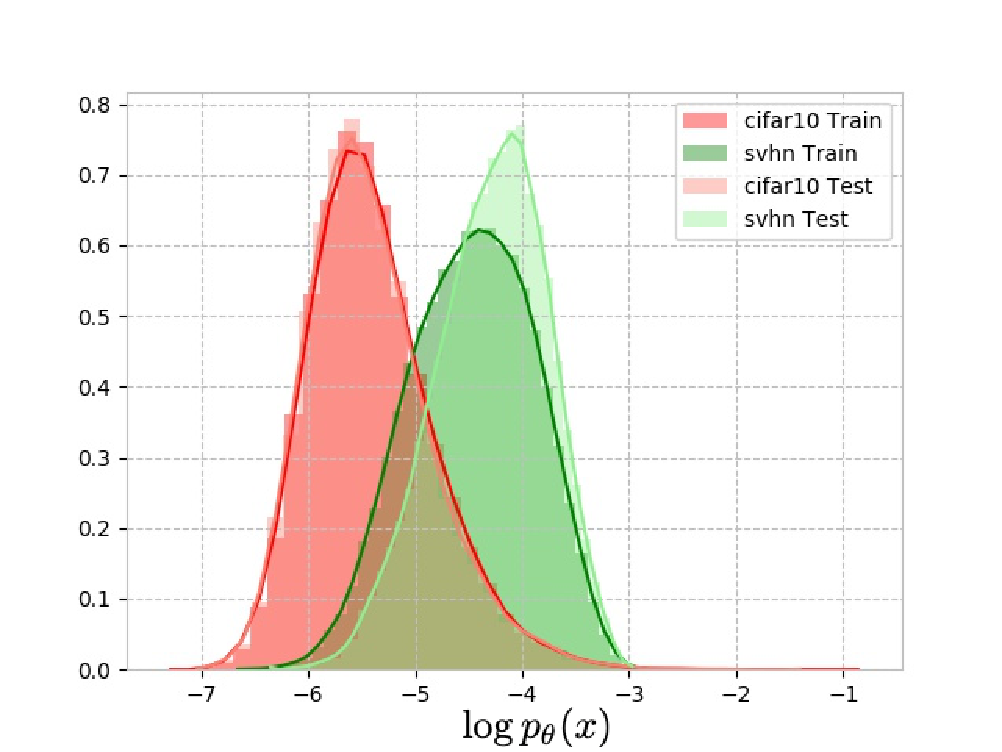
\includegraphics[width=0.45\columnwidth]{counterexample1}
}
\subfigure[KMNIST vs Omniglot]{
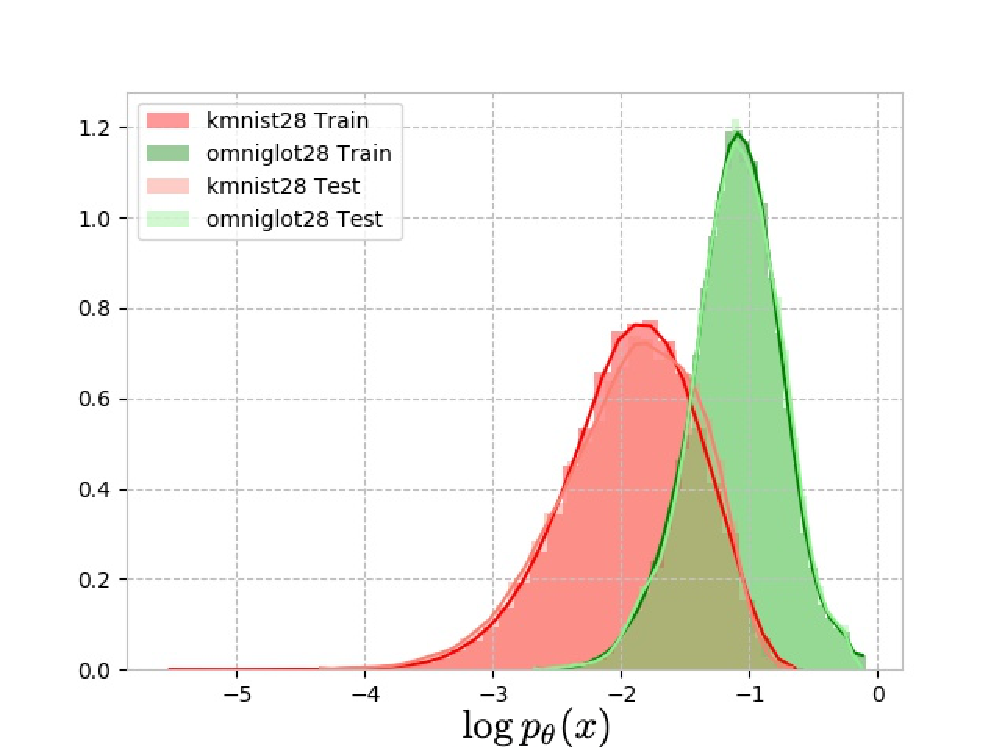
\includegraphics[width=0.45\columnwidth]{counterexample2}
}
\quad
\subfigure[SVHN vs CIFAR-10]{
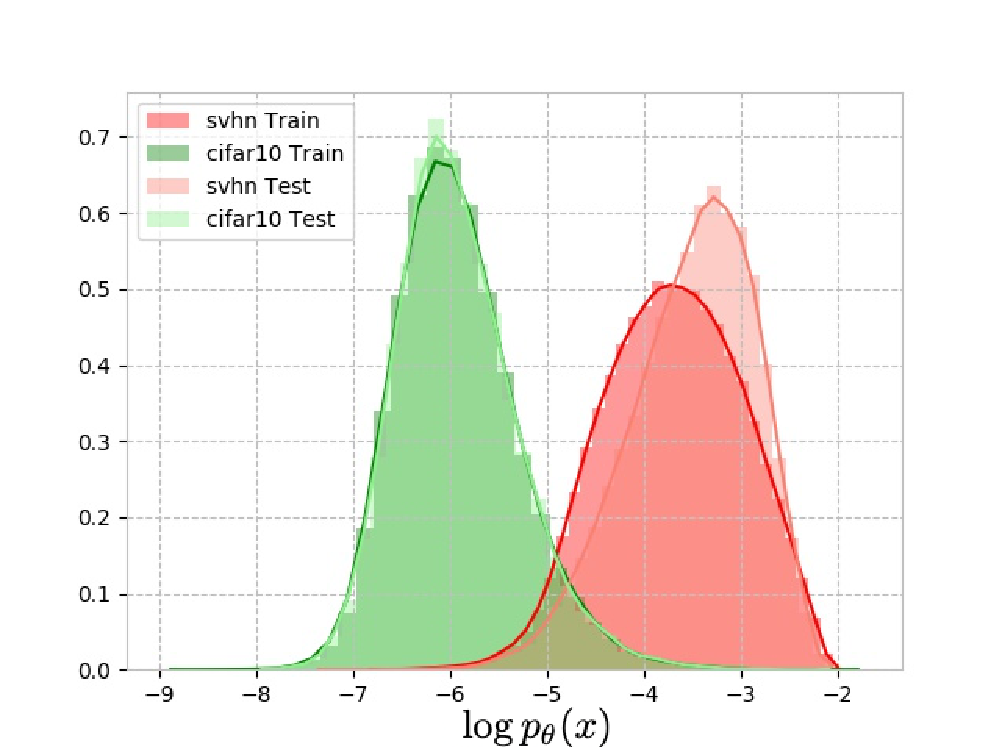
\includegraphics[width=0.45\columnwidth]{counterexample3}
}
\subfigure[MNIST vs Omniglot]{
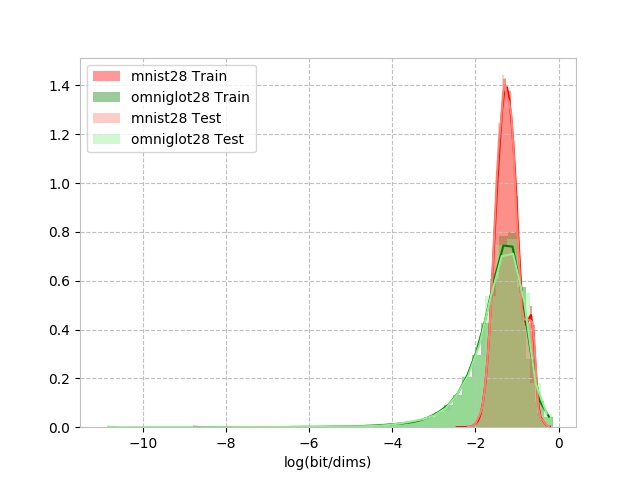
\includegraphics[width=0.45\columnwidth]{counterexample4}
}
\caption{The log-likelihood of VAE. The AUROC of log-likelihood in (a) (b) (c) (d) are 0.08, 0.09, 0.99, 0.59. The AUROC of T-perm in (a) (b) (c) (d) are 0.84, 0.82, 0.98, 0.66. These experiments show that log-likelihood of out-of-distribution might be higher, lower or nearly same to the log-likelihood of in-distribution.}
\label{fig1}
\end{figure}

\subsection{Counterexamples}
The log-likelihood of likelihood-based models is expected to be lower in the out-of-distribution and be higher in the in-distribution intuitively, because the models are trained at in-distribution. 
However, the observation of \cite{nalisnick2018deep} shows that all of models give the higher log-likelihood at out-of-distribution in experiments CIFAR-10 vs SVHN and NotMNIST vs MNIST. 
We observed that the number of datasets in \cite{nalisnick2018deep} is quite small and we suspect that there might be more counterexamples at large-scale datasets. 

Therefore, we reproduce the experiments at more datasets and find more counterexamples shown in \ref{fig1} and appendix A. 
These experiments show that log-likelihood is unpredictable at out-of-distribution, \IE it might be lower, higher or same. 
Moreover, the methods based on the log-likelihood might have counterexamples at large-scale datasets. 
We reproduce the indicators~\cite{alemi2018uncertainty,song2017pixeldefend,ren2019likelihood,song2019generative,nalisnick2018deep,che2019deep,alemi2018uncertainty} on common generative models and find counterexamples at large-scale datasets, shown in appendix A. \cite{nalisnick2018deep} observed that there is a clear negative correlation between likelihoods trained on CIFAR-10 and FashionMNIST and their complexity estimates over large-scale datasets. We validate their observation over large-scale datasets. However, such correlation is depend on the in-distribution. It matters the performance of indictors as shown in \cref{fig2}. 

\begin{figure}[t]
\centering
\subfigure[Correlation]{
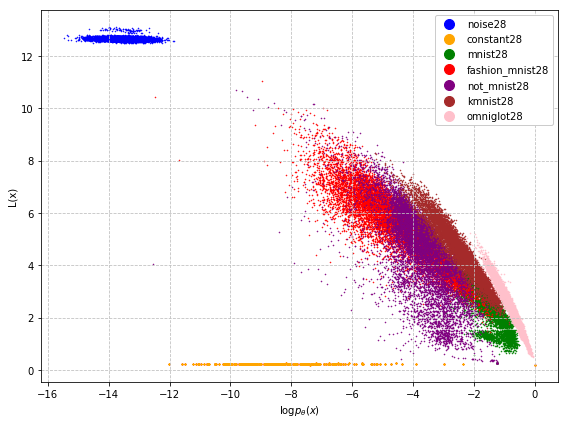
\includegraphics[width=0.45\columnwidth]{counterexample_complexity1}
}
\subfigure[AUROC = 0.9867]{
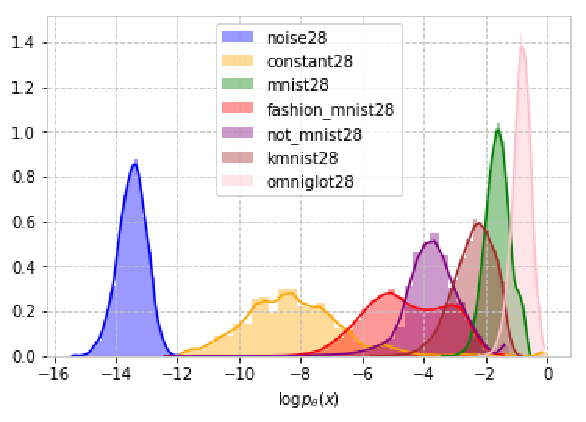
\includegraphics[width=0.45\columnwidth]{counterexample_complexity2}
}
\subfigure[AUROC = 0.7770]{
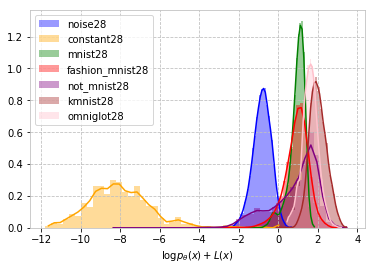
\includegraphics[width=0.45\columnwidth]{counterexample_complexity3}
}
\subfigure[AUROC = 0.9999]{
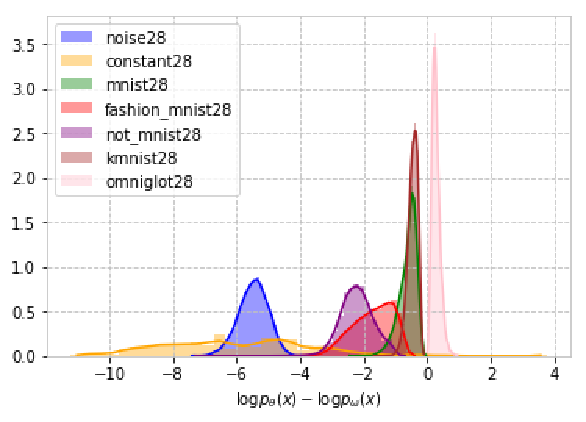
\includegraphics[width=0.45\columnwidth]{counterexample_complexity4}
}
\caption{We select Omniglot as in-distribution and other grey datasets as out-of-distribution. (a) shows the correlation between likelihoods trained on Omniglot and complexity estimate. (b) shows the histogram of log-likelihood. The average AUROC over all testing datasets is 0.9867. (c) shows that indictor $S(x)$ might reach lower the performance than log-likelihood. It means that $L(x)$ is rough and we need a more precise, stable and interpretable estimate to assist log-likelihood for detecting OoD. (d) shows $\log p_\theta(x) - \log p_\omega(x)$ might be a good choice where $p_\omega$ is trained on out-of-distribution.%(e) TODO shows that the density of samples on out-of-distribution increase instead decrease during training. 
}
\label{fig2}
\end{figure}

\subsection{Performance on Large-scale Datasets}
Based on the following reasons, we use the large-scale datasets instead few datasets to check the generality of indicators:

\begin{itemize}
	\item The critical reason is that their indictors are supported by the motivating observation on few datasets, instead of the theoretical proof, however, the datasets in the past works are too less to validate the generality of motivating observation. 
	\item The performance on few datasets might be early improved by fine-tuning hyper-parameters and architectures of models but not on large-scale datasets. 
	\item By the definition of OoD problem in \cref{sec2}, models should distinguish any $\pout$ that is distinct to $\pin$ instead of few datasets. Therefore, we should check more out-of-distribution as much as possible. 
	\item Average performance on large-scale datasets is better for assessing indictors. In CelebA vs LSUN, log-likelihood reach 0.98 AUROC (1.0 is best), however, our counterexamples show that it gets 0.02 in CelebA vs SVHN. Average performance will consider such experiments with lower AUROC. We think that it is more meaningful to improve the average performance of indictors rather than improve little in a single experiment. 
\end{itemize} 


Our experiments in \cref{table1} show that on large-scale datasets the performance of the indictors of past work via common deep generative models are not good as they claimed. 

\subsection{Observation of KL indicator}
As shown in \cref{fig2}, complexity estimate is unstable and sometimes it might lower the performance. Therefore, we try to find another function to replace the term $L(x)$ in $S(x)$. 
In our experiments over large-scale datasets, we observe a phenomenon that $p_\theta(x) < p_\omega(x)$ for almost $x \sim \pout$ and $p_\theta(x) > p_\omega(x)$ for almost $x \sim \pin$ where $p_\omega(x)$ is a model trained on out-of-distribution. The average AUROC of $p_\theta(x) - p_\omega(x)$ reaches nearly 1.0 over all datasets, as shown in \cref{table1}.
From the view of complexity estimate, $L(x) = -\log_2 p(x|\mathcal{M}_0)$ can be regard as a log-likelihood of a universal model $\mathcal{M}_0$~\cite{serra2019input}. In our paper, $p_\omega(x)$ is used to replace $L(x)$ for assisting log-likelihood. 

However, in OoD problem, we are not allowed to know any information of the out-of-distribution. 
Therefore, we will explore how to develop an indictor that are not depend on a model trained on out-of-distribution and why $p_\theta(x) - p_\omega(x)$ is almost useful for OoD theoretically. 

\section{Native Indicators}
\subsection{Basic Native Indicators}
In the definition of OoD problem, we do not give any assumption about the probability distribution, since we try to make the definition more general. Our theory are based on following assumption about the probability distribution for OoD problem:
\begin{enumerate}
	\item The training data and testing data in in-distribution and out-of-distribution are i.i.d. 
	\item There exists a divergence $div$, satisfying that $div(\pin, \pout) \gg 0$ and $div(\pout, \pin) \gg 0$. 
	\item If $div(\pin, \pout)$ and $div(\pout, \pin)$ can be represented by sampling formula, \IE $div(\pin, \pout) \approx \sum_{i} f(x_i)$, then $f(x_i) \gg 0$ for almost  $x_i$. 
	\item $f: \mathcal{X} \rightarrow \mathcal{R}$ maps the distribution $\pin, \pout$ into two Gaussian distribution with constant variance. 
	\item 3 and 4 holds for any indictor $\hat{f}$ approximating $f$. 
\end{enumerate} 

It is important to notice that assumption 3 can not be deduced from assumption 2 obviously. For example, when $\pin = \frac{1}{2}(\mathcal{N}(0, 1) + \mathcal{N}(-10, 1))$ and $\pout = \frac{1}{2}(\mathcal{N}(0, 1) + \mathcal{N}(10, 1))$, $KL(\pin, \pout) \approx 25.05 \gg 0$ but $\log \pin(x) - \log \pout(x) \approx 0$.  In such example, $\pin$ and $\pout$ is distinguishing by KL-divergence but is not simply classified because no classier can detect whether a sample in $\mathcal{N}(0, 1)$ is from $\pin$ or $\pout$. We assume that assumption 3 holds when $\pin$ and $\pout$ is simply classified. 

Above assumption means that if $D$ can distinguishing the probability distribution                                                                                                        in-distribution and out-of-distribution, then $f$ can be used as an indicator for detecting whether a sample is OoD. $f$ is called the Native Indictor based on $D$. 

For detailed research, \EG how to use native indictor when we do not know out-of-distribution, we need more property of $div$. 
We will introduce two kinds of Native Indictors: Native KL Indictor and Native Wasserstein Indictor. 

\subsection{Native KL Indicator}
We select KL-divergence as $D$, then $KL(\pin, \pout) = \E_{\pin(x)} [\log \pin(x) - \log \pout(x)]$ and Native KL Indictor is $\log \pin(x) - \log \pout(x)$. \cref{fig3} interprets the motivation of native KL indictor. 
\begin{figure}
	\center
	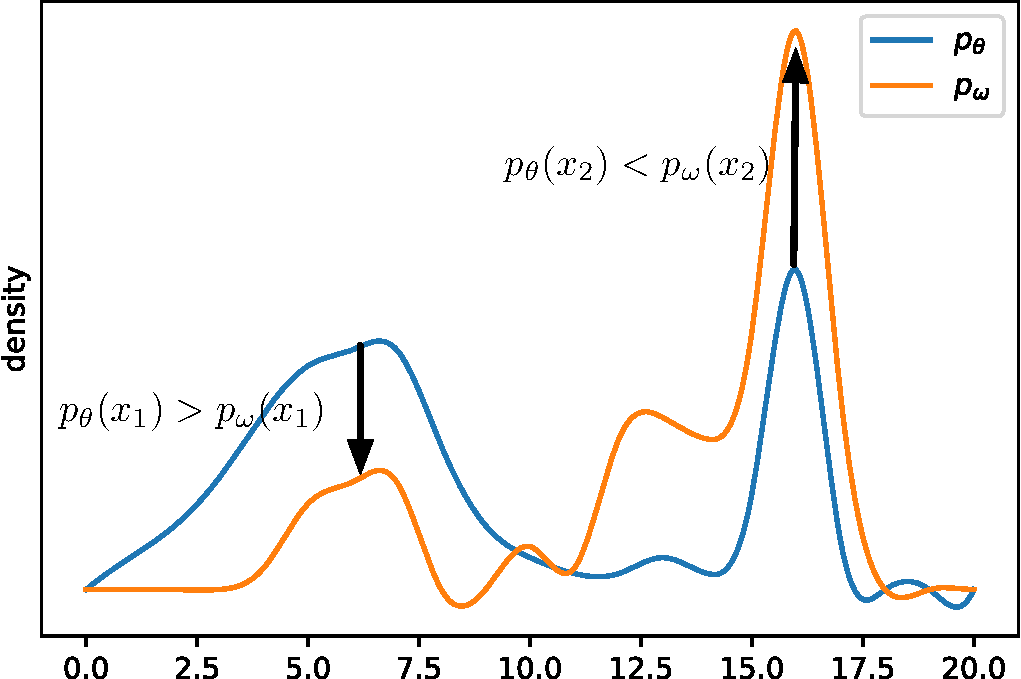
\includegraphics[width=0.9\columnwidth]{diagram}
	\caption{Diagrammatic sketch for the motivation of Native KL Indictor. The in-distribution is in [0, 10] and out-of-distribution in [10, 20]. Intuitively, $p_\theta$ has a lower density for samples from in-distribution and higher density for samples from out-of-distribution than $p_\omega$ . 
	Different to the assumption of log-likelihood indictor, we do not assume that $p_\theta(x_2)$ or $p_\in(x_2)$ is a very lower density for $x_2 \sim \pout$. By the assumptions, we can induce that $\pin(x_1) < \pout(x_1)$ and $\pin(x_2) > \pout(x_2)$. $p_\theta$ and $p_\omega$ also have this property, \IE $p_\theta(x) - p_\omega(x)$ is an indictor for OoD detection. }
	\label{fig3}
\end{figure}

\begin{theorem}\label{thm1}
	$\log \pin(x) - \log \pout(x)$ is a symmetric indictor, \IE it reaches same performance in experiment A vs B and B vs A, with a natural threshold zero. 
\end{theorem}
Likelihood is not a symmetric indictor since it uses $p_A$ as indictor in experiment A vs B and $p_B$ as indictor in experiment A vs B. An interesting phenomenon is that if likelihood indictor reaches a good performance on experiment A vs B, then it will usually fail in experiment B vs A, in appendix B. A special example is the experiment of Noise vs any dataset. The optimal model of Noise dataset is uniform distribution, however, it can not detect any OoD. In the experiment of any dataset vs Noise, likelihood reaches nearly best performance since the log-likelihood of noise is significantly lower than any datasets. 

However, $\pout$ is unknown under the limitation of OoD problem. Therefore, we try to use another tractable term to replace $\pout$. 

\begin{theorem}\label{thm2}
	For any mixture distribution $\pmix = \alpha \pin + \beta \pout$ where $\alpha + \beta = 1$ and $\alpha, \beta > 0$, the performance of indictor $\log \pin(x) - \log \pmix(x)$ and indictor $\log \pin(x) - \log \pout(x)$ are equal for OoD detection. 
\end{theorem}

If we can get enough data from the mixture distribution, By \cref{thm1}, a model $p_\gamma$ that is trained to approximate $\pmix$ can be used to replace the term $\pout$ in Native KL Indictor and ensure the same performance. It is also observed in our experiments, shown in \cref{tab1}. Next, we try to explain why native KL indictor can reach outstanding performance.

Compared to log-likelihood indictor and likelihood-ratio indicator, Native KL Indictor can always get better performance. 
\begin{theorem}\label{thm3}
By the assumption that log-likelihood can detect OoD, $\log \pin(x_1) > \log \pin(x_2)$ for almost $x_1 \sim \pin$ and $x_2 \sim \pout$. At such situation, assumption 3 can be deduced, \IE Native KL Indictor can be also used to detect OoD. 
\end{theorem}

\begin{theorem}\label{thm4}
For any likelihood-ratio indictor in formula $\log \pin(x) - \log g(x)$ where $g$ is a continuous differentiable probability distribution, Native KL Indictor outperforms them in OoD problem with suitable mathematical simplification. 
\end{theorem}

By above theorems, we show that Native KL Indictor can be obtained by mixture distribution. It is natural to use two modeled distribution to model in-distribution and mixture distribution. 

Next, we will show the property of modeled distribution. Let $p_\theta, p_\gamma$ models $\pin, \pmix$, \IE $\theta = \arg \max_\theta \E_{\pin(x)} \log p_\theta$ and $\gamma = \arg \max_\gamma \E_{\pmix(x)} \log p_\omega$. $\log p_\gamma(x) - \log p_\theta(x)$ acts as the indictor. 

\begin{theorem}\label{thm5}
	$\log p_\theta(x) - \log p_\gamma(x)$ can be used for detecting OoD, only requiring that the training converges, without the condition that $p_\theta$ sufficiently approaches $\pin$ and $p_\gamma$ sufficiently approaches $\pout$ with suitable mathematical simplification. Moreover, $\log p_\theta(x) - \log p_\gamma(x)$ reflects whether a sample $x$ in mixture distribution have been optimized in the training process of $\theta$. 
\end{theorem}

\cref{thm4} shows $\log p_\theta(x) - \log p_\gamma(x)$ reflects the optimizability: if a sample $x$ is OoD, then $p_\theta(x)$ will be lower than $p_\gamma(x)$ since $x \sim \pmix$ and $\gamma$ can optimize $x$ more than $\theta$. By \cref{thm4}, we will not require that $\theta$ approach $\pin$ sufficiently and $\gamma$ approach $\pmix$ sufficiently but only the training of $\theta$ and $\gamma$ converges. It alleviates the requirements for training and then we can discuss how to train models on online system. 

\subsection{Native Wasserstein Indicator}
In \cite{nalisnick2018deep}, they do not include GANs in the comparison since how to evaluate the density of GANs is an open problem. Some researches propose  variants of GANs with tractable density~\cite{kumar2019maximum}. In the framework of Native Indictors, we can detect OoD by GANs without the density of GANs. 

In vanilla GAN~\cite{goodfellow2014generative}, a discriminator is trained to distinguish generated samples and real samples and  a generator is trained to generate samples for deceiving the discriminator.

However, vanilla GAN is unstable during the training process. To tackle this problem, Wasserstein distance is introduced by WGAN~\cite{arjovsky2017wasserstein}:
\begin{equation}
	W^1(\mu, \nu) = \sup_{Lip(D) \leq 1} \{\E_{\mu(x)} D(x)  - \E_{\nu(x)} D(x)\}
\end{equation}

We select Wasserstein distance as $div$, then
\begin{equation}
	W^1(\pin, \pout) \approx \sum_i \Big[D(x_i^{in}) - \sum_j D(x_j^{out})\Big]
\end{equation} 
where $x_i^{in}$ is sampled from in-distribution and $x_j^{out}$ is sampled from out-of-distribution and $D$ is the optimal solution in $W^1(\pin, \pout)$. Then the Native Wasserstein Indicator for sample $x$ is $D(x) - \sum_{j} D(x_j^{out})$. Notice that $\sum_{j} D(x_j^{out})$ is a constant and it will not affect the performance of OoD detection. Therefore, the Native Wasserstein Indicator is simply $D(x)$. The generator of WGAN does not appear in our formula since we only consider how to measure the distance between $\pin, \pout$ instead of generating. 

Similar to Native KL Indicator, we will show some theorems to show the property of Native Wasserstein Indicator to ensure that it can be obtained without any information of $\pout$. 

\begin{theorem}\label{thm6}
	Assumption 2 is a corollary of definition of OoD problem when $div$ is Wasserstein distance.  
\end{theorem}

\begin{theorem}\label{thm7}
	$D(x)$ is a symmetric indictor. 
\end{theorem}

\begin{theorem}\label{thm8}
	$\hat{D}$ that is optimal solution in $W^1(\pin, \pmix)$ is same to the optimal solution $D$ in $W^1(\pin, \pout)$. 
\end{theorem}

Because the Native Wasserstein Indicator is only depend on $D$, by \cref{thm5} we could use $\hat{D}$ that is independent to $\pout$ to replace $D$. 

\begin{theorem}\label{thm9}
	The discriminator in $W^1(\pin, \pout)$ is the best indictor among all indictors that is 1-Lipschitz. Moreover, it is the best indictor who has limited gradient. 
\end{theorem}

\subsection{Concerns}
We have proposed a method to exploit the samples of mixture distribution to train a model for OoD detection. However, there are three major concerns about this idea: 
\begin{itemize}
	\item Is this method \textbf{data-specific}? \IE does this method only work on the data that it has seen in training? 
	\item Can this method work on \textbf{online system}? \IE for a new testing data, model should give the indictor before the next texting data comes.  
	\item Can this method works only with \textbf{a batch of samples}? \IE model must detect immediately while it only knows in-distribution data and a batch of mixture distribution. 
	\item Is it better to train \textbf{pre-train} models (trained on in-distribution) or \textbf{initialized} models on on mixture distribution?
\end{itemize} 

To solve the concerns, we design following experiments:
\begin{itemize}
	\item In experiment A vs B, only 20\% data in mixture distribution can be used for training. 
	\item We simulate the online system --- the data in mixture distribution is streaming and requires the indicator immediately. 
	\item We splits the data from mixture distribution into several batches and model can only know the in-distribution and the batch that it is detecting. 
	\item Experiments for pre-train models and initialized models. 
\end{itemize}

\section{Experiments}
In this section, we will demonstrate the effectiveness of Native KL Indictors and Native Wasserstein Indictors on several computer vision benchmark datasets. We run all experiments with Pytorch and Tensorflow and we submit the code to reproduce all experimental results. 

\subsection{Datasets}
All the datasets considered are listed below:
\begin{enumerate}
	\item \textbf{CIFAR-10} is a natural image datasets with 10 classes including animal, ship, airplane and etc. 
	\item \textbf{CIFAR-100} is just like CIFAR-10, including 100 classes. 
	\item \textbf{SVHN} includes house numbers from 0 to 9. 
	\item \textbf{CelebA} is a large-scale face attributes dataset. 
	\item \textbf{TinyImageNet} consists of a subset of ImageNet images. It contains 200 different classes.
	\item \textbf{LSUN} has a testing set of 10 different scenes. 
	\item \textbf{iSUN} is subset of SUN, including 8925 scene images in 899 different scenes.
	\item \textbf{MNIST} consists of handwritten digits from 0 to 9. 
	\item \textbf{Fashion MNIST} includes 10 kinds of clothes and shoes. 
	\item \textbf{Not MNIST} includes letters from A to J on various typefaces. 
	\item \textbf{KMNIST} includes 10 kinds of Kanji characters.
	\item \textbf{Omniglot} contains 1623 different handwritten characters from 50 different alphabets. 
	\item \textbf{Noise} is created by uniformly randomly sampling. 
	\item \textbf{Constant} includes images whose pixels have same color. 
\end{enumerate}

The natural images are resized into 32x32x3 and grey images are all 28x28x1. All pair in natural image datasets and all pair in grey image datasets are considered in our experiments. Only CIFAR-10, CIFAR-100 and TinyImageNet are not simply-classified and in fact they have similar classes. Noise and Constant includes both grey and natural images. LSUN (only including testing data) and iSUN are only used for out-of-distribution. 

CelebA, Noise and Constant have no labels, thus we create random labels whose value in 0-9 on these datasets. 

\subsection{Metrics}
Following metrics are adopted to measure the effectiveness of a method in out-of-distribution detection:
\begin{itemize}
	\item \textbf{AUROC} is the Area Under the Receiver Operating Characteristic curve, which is a threshold-independent metric~\cite{davis2006relationship}. AUROC can be interpreted as the probability that a sample from in-distribution is assigned a lower detection score than a sample from out-of-distribution~\cite{fawcett2006introduction}. It is widely applied in OoD domain. We select AUROC as our major metrics. 
	\item \textbf{AUPR} is the Area under the Precision-Recall curve, which is another threshold independent metric~\cite{saito2015precision}. AUPR-In and AUPR-Out denotes the AUPR where in-distribution and out-of-distribution are positive, respectively.  
	\item \textbf{AP} is the Average Precision. AP summarizes a precision-recall curve as the weighted mean of precisions achieved at each threshold. 
	\item \textbf{FPR@TPR95} is the False Positive Rate when True Positive Rate is over 95\%. It means the probability that an out-of-distribution example is misclassified as in-distribution when over 95\% in-distribution is detected accurately.
\end{itemize} 

\subsection{Setups} 
For fair comparison, all indictors are based on common models with standard training, including 34-layer ResNet, VAE, PixelCNN, Glow and Wasserstein GAN. ResNet34 is trained to classify the in-distribution and out-of-distribution for validate whether they are simply classified. ResNet34 is also trained for classification and serves for the OoD indictors based on classifier. Deep generative models are trained as their proposer suggests without any other tricks. 

In our experiments, there are not validation set. For the indictors depending on hyper-parameters, we try grid-searching as their proposers suggest and report the performance with all hyper-parameters considered. To ensure the generality over all datasets, it is forbidden to specify the hyper-parameters or architectures on any dataset. 
The detailed architecture and parameters are shown in appendix B. 

\subsection{Major Results}

The main results for indictors of past works are summarized in \cref{tab1}. The main results for Native KL Indictor and Native Wasserstein Indictors are summarized in \cref{tab2}. 

\subsection{Validation of Theorem}

\cref{thm1} is supported by the detail experiments shown in appendix B. \cref{thm2} is supported by the performance of native KL indictor based on mixture distribution. 
\cref{fig4} shows that native KL indictor can also get same performance when log-likelihood can reach outstanding performance, to support \cref{thm3}. 

\begin{figure}
	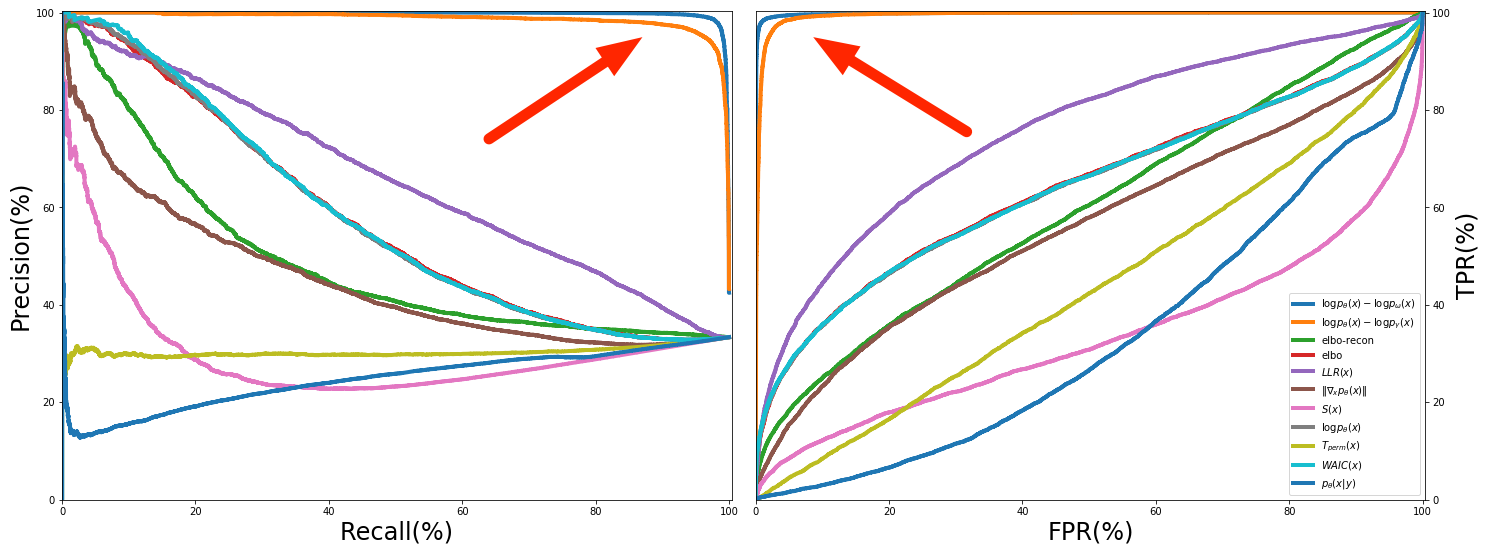
\includegraphics[width=1.0\columnwidth]{roc_prc}
	\caption{ROC and Precision-Recall Curve on CIFAR-100 vs CelebA based on VAE model. The native KL Indictor outperforms other indictors. }
	\label{fig5}
\end{figure}

We compare the precision-recall curve and ROC curve of native KL indictor, log-likelihood indictor, likelihood ratio indictor and log-likelihood with input complexity in \cref{fig5}, to show native KL indictor is the best version of log-likelihood ratio indictor, to support \cref{thm4}. \cref{fig6} shows the change of AUROC during training on mixture distribution to support \cref{thm5}. 

\cref{thm7} is supported by the detail experiments shown in appendix B. In table \cref{tab2}, the performance of the native Wasserstein indictor trained on mixture distribution is near same as the native Wasserstein indictor trained on out-of-distribution, which validates \cref{thm8}. The outstanding performance of the native Wasserstein indictor supports the \cref{thm9}. 

\subsection{Concerns}

The experiments about concerns are showing in \cref{tab3}. \cref{fig8} shows the change of AUROC while the size of batch varies. These experiments show that native KL indicator and native Wasserstein indictor are effective, robust, general, online and not data-specific. It also show the weakness of these native indictors that it can not work well when only a few data from mixture distribution is provided. 

\section{Limitations of the Study} In this section, we will discuss the limitation of our paper in datasets, models and native indictors. 

\subsection{Limitation of datasets}
In our paper, we try large-scale datasets to show the generality of indictors. However, we only consider natural OoD datasets \cref{chen2020robust} and do not consider attacked OoD. An important reason is that it is quite hard to design a principle like simply classified, to measure these attacked OoD datasets. 

\subsection{Limitation of models} 
In our paper, for fair comparison and the research for generality, we only consider the common models, including ResNet, VAE, PixelCNN, Glow and WGAN. However, there are numerous models careful-designed for OoD detection. Limited by our computation resource, we can not give the performance of them over large-scale datasets. 
We have emphasized that it is unreliable to evaluate the models for OoD in a few datasets in this paper and we expect that it can become a common sense in OoD domain. 

\subsection{Limitation of native indictors} 
While native indictors show outstanding performance in our experiments, we have also observed some defects of them. They depend on the model (\EG Native KL Indicator based on Glow is data-specific) and optimizer (\EG when data from mixture distribution is not enough for training, optimizer can not give the expected $p_\gamma$ expect). It is natural to design an indicator to approximate $\log p_\gamma(x) - \log p_\theta(x)$ without optimizer, \EG by Taylor Expansion. We leave it for future work. 
Native indictors will lead to many works since it rise simply, fundamental and practical indictors with solid experiments and theories. 

\section{Conclusion and Future Work}


\bibliography{reference.bib}

\appendix
\section{Counterexamples}
\section{Experiemtns}
\section{Proof}
\end{document}
